\documentclass[10pt,a4paper]{article}
\usepackage[margin=17mm]{geometry}\usepackage{fontspec,amsmath,graphicx,booktabs}
\setmainfont{Latin Modern Roman}\setlength{\parindent}{0pt}\setlength{\parskip}{6pt}
\begin{document}
{\LARGE Reference distribution tests}\par 6 October 2026

\textbf{Result.} Uniform arc resampling of the final averaged reference and arc weighting of the original points give similar physical fits. The simple direct-inversion sphere-circle guide does not provide a reliable monotone phase coordinate here: making it monotone largely removes the inner loop from the averaged reference. This is a reference-construction failure, not evidence that a physical background model fits better.

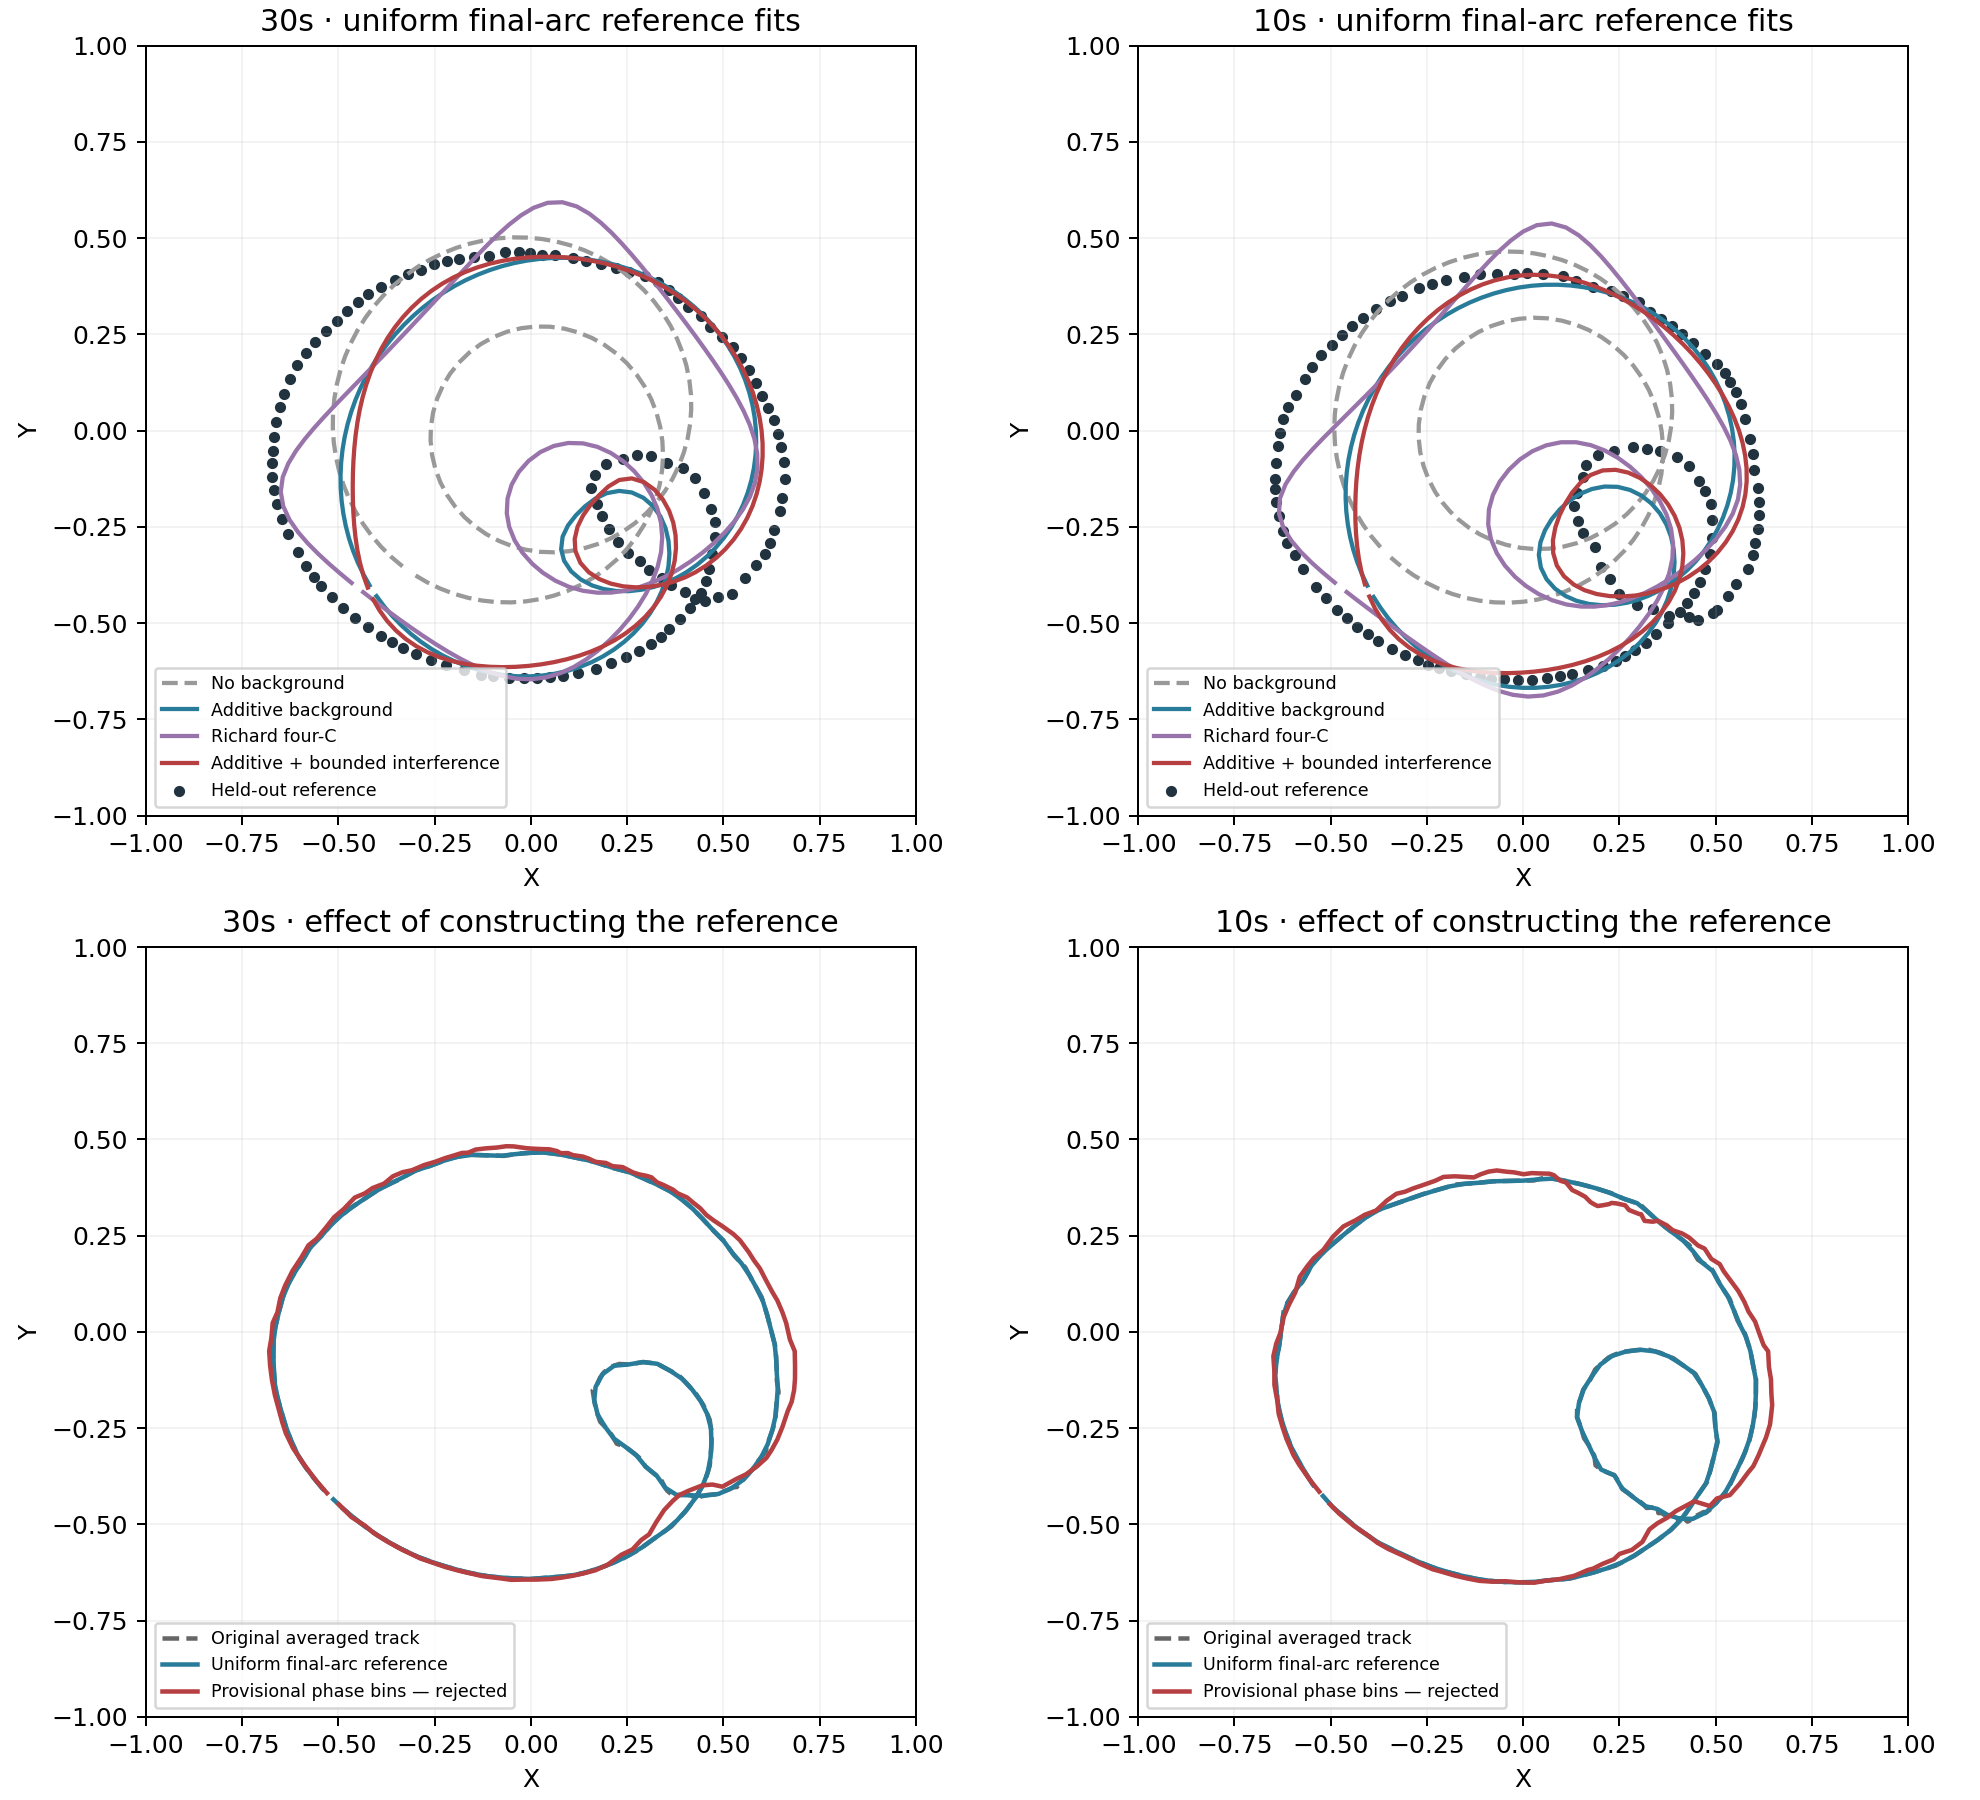
\includegraphics[width=\linewidth,height=.82\textheight,keepaspectratio]{sampling_comparison.png}
\newpage
{\Large Primary comparison: weighting versus resampling}

Two tests isolate the uneven-density concern. Weighted: preserve all original intensities and use trapezoidal arc weights. Uniform: interpolate the four channels together to 128 equally spaced locations along the final training-average arc; apply the identical training-derived interpolation map to the held-out average. Simulation is always matched using actual final-reference arc coordinates, one cyclic offset and both directions. No flexible phase warp.

\[
J=\sum_k w_k\sum_i\left[\frac{I_{i,k}^{\rm pred}-I_{i,k}^{\rm obs}}{T_k^{\rm obs}}\right]^2,
\quad w_k\propto\frac{\Delta s_{k-1}+\Delta s_k}{2}.
\]
For the uniform reference, bin weights are equal. To compare the two fitted models fairly, the table below evaluates both on the \emph{same original held-out intensities with the same arc weights}. Their starting reference point is identical; no extra held-out alignment is fitted.

\begin{tabular}{llrrrr}\toprule
Window & Model & Weighted fit & Uniform fit & Uniform BG/\(T_{\max}\) & Uniform \(\theta\)\\\midrule
30s & None & 0.07633 & 0.07633 & 0.0\% & 30.3--46.8$^\circ$ \\
30s & Additive & 0.02856 & 0.02857 & 35.5\% & 29.1--89.9$^\circ$ \\
30s & Richard four-C & 0.03876 & 0.03876 & --- & 29.0--88.6$^\circ$ \\
30s & Additive + interference & 0.02612 & 0.02613 & 42.4\% & 30.0--90.0$^\circ$ \\
10s & None & 0.07524 & 0.07526 & 0.0\% & 31.3--45.0$^\circ$ \\
10s & Additive & 0.03217 & 0.03208 & 38.3\% & 33.7--89.9$^\circ$ \\
10s & Richard four-C & 0.03883 & 0.03879 & --- & 33.4--88.4$^\circ$ \\
10s & Additive + interference & 0.02872 & 0.02860 & 39.8\% & 34.3--89.9$^\circ$ \\
\bottomrule\end{tabular}

Both preserve the measured two-loop trajectory. The residual mismatch remains after removing uneven-density weighting. This supports using the simpler uniform-final-arc reference for presentation and retaining arc weighting as a control. It does not prove the physical models or angles correct.

All four models retain fixed excitation with one brightness scale, original optics/calibration, and the same background budget in original intensity units. The additive budget is held fixed at 95\% of the original training minimum across reference methods, rather than changing the budget when resampling changes a sampled minimum. Physical curves are not used to replace measured points. Mean-of-channel values are retained before calculating anisotropy.

Richard uses the stable equivalent parameterization \(I_i=\alpha f_i+K_i\sqrt{f_i}\), with \(\alpha=a_0^2\), \(K_i=a_0C_i\). Under these new arc-weight objectives the selected alpha values are finite (about 0.0192/0.00511 for uniform 30/10 s). The previously reported zero-brightness tendency therefore depends on weighting; the structural degeneracy of the unconstrained model has not been removed.

Nine base starts per model/window/reference cover both directions and four offsets, plus nested-model starts. Selected primary fits converge and have positive predicted channels. Local optimality is not a global guarantee. Uniformity refers to integrated arc on the reference interpolant; adjacent straight chord lengths need not be identical at curved sections.
\newpage
{\Large Direct-inversion sphere-circle phase guide}

Raw calibrated channels from 30--31 s and 10--11 s were checked: \textbf{zero samples outside the nominal inversion domain} in either 250,000-sample window. The user's expectation about the range is supported on these data. A 41-sample channel smoother constructs the guide only; it does not replace the intensities being averaged.

For each ordered cycle, invert guide anisotropy to folded theta and unwrapped phi. Fit one provisional least-squares plane using equally weighted training cycles (128 time-decimated guide directions each). Project directions into that plane's basis and unwrap their polar angle. This circle/plane sets a coordinate only; neither its cone geometry nor its projected points enter the physical fit as measured data.

The coordinate reverses substantially within individual traversals. Normalizing the first-to-last angle span to one traversal does not remove these reversals. A monotone least-squares (isotonic) guide was tried as a deliberately flagged sensitivity, while preserving acquisition order. Raw channel means in the resulting contiguous bins were then averaged with equal cycle weight. No cycles were removed (304 total, 152/152 split; 217 total, 109/108 split).

\begin{tabular}{lrr}\toprule
Guide diagnostic & 30--31 s & 10--11 s\\\midrule
Median maximum monotone adjustment & 15.0\% & 21.7\%\\
95th percentile maximum adjustment & 28.3\% & 39.1\%\\
Median adjustment with separate plane per cycle & 15.4\% & 22.4\%\\\bottomrule
\end{tabular}

These are fractions of each normalized provisional traversal, not angular measurement errors. The median raw plane-angle span is only about 0.53--0.54 turns per detected track. The uncorrected anisotropy winds once around the origin, so its half-angle inversion does not yield a closed directed upper-hemisphere trajectory. This is a limitation of this simple uncorrected guide, not an assertion that phase guidance can never work.

The guide is not one-to-one through the inner loop. Flattening its reversals concentrates different trajectory sections into a small phase region; averaging then largely erases the inner loop (bottom row of figure). This occurs even though every raw intensity sample is retained in some bin and no intensity is replaced by a circle prediction.

\textbf{Disposition.} Fits on the phase-binned references were completed as diagnostics, saved in fits.json/summary.csv, and explicitly excluded from the primary comparison. They should not be interpreted as corrected rod angles or improved fits. The 10 s complex phase-reference run also exhausted its refinement budget; no conclusion relies on its optimum. A separate best plane per cycle did not cure the guide-coordinate instability. No extra fitted phase flexibility or new inverse-circle constraints were introduced.

Files: prepare.py (raw reference construction), fit.py (24 model/reference/window fits), report.py, references.npz, preparation\_checks.json, additional\_guide\_checks.json, fits.json and summary.csv. Reproduce using numpy/scipy/matplotlib/nptdms; XeLaTeX builds this report. No commit or push.
\end{document}
